%\newcommand{\eps}{\epsilon}
\newcommand{\Pmax}{p_\text{max}} 	
\newcommand{\Hint}{H_{int}}
\newcommand{\kbar}{\bar{k}}
\newcommand{\Delk}{\Delta}
\newcommand{\Sumk}{\Sigma}
\newcommand{\Qrot}{Q_{pq}(\tau_s)}
\newcommand{\shapecor}{\mathcal{S}}
\newcommand{\ampcor}{\mathcal{A}}
\newcommand{\totalcor}{\mathcal{E}}
\newcommand{\threeLs}{L_p(\kbar_1)L_q(\kbar_2)L_r(\kbar_3)}
\newcommand{\threePs}{P_p(\kbar_1)P_q(\kbar_2)P_r(\kbar_3)}
\newcommand{\threeQs}{Q_p(k_1)Q_q(k_2)Q_r(k_3)}
\newcommand{\Lbasic}{\mathcal{P}_0}
\newcommand{\Linvk}{\mathcal{P}_1}
\newcommand{\Lnsinv}{\mathcal{P}^{n_s}_1}
\newcommand{\Lnsboth}{\mathcal{P}^{n_s}_{01}}
\newcommand{\Linvksq}{\mathcal{P}_2}
\newcommand{\Lns}{\mathcal{P}^{n_s}_2}
\newcommand{\Fbasic}{\mathcal{F}_0}
\newcommand{\Finvk}{\mathcal{F}_1}
\newcommand{\Finvksq}{\mathcal{F}_2}
\newcommand{\quadpot}{V_{\phi^2}(\phi)}
%\newcommand{\threeqs}{q_p(\kbar_1)\,q_r(\kbar_2)\,q_s(\kbar_3)}
\newcommand{\threeqs}{q_p(k_1)\,q_r(k_2)\,q_s(k_3)}
\newcommand{\threeqstilde}{q_{\tilde{p}}(k_1)\,q_{\tilde{r}}(k_2)\,q_{\tilde{s}}(k_3)}
\newcommand{\kmin}{{k_\text{min}}}
\newcommand{\kmax}{{k_\text{max}}}
\newcommand{\fnl}{f_{NL}}
\newcommand{\fnllocal}{f^{local}_{NL}}
\newcommand{\fnlequil}{f^{equil}_{NL}}
\newcommand{\fnlortho}{f^{ortho}_{NL}}

\chapter{Constraints}\label{chapter:constraints}
\section{Connecting to $\cmbbest$}
\textcolor{red}{We don't get an exact match, maybe due
to $140$ Gaussian simulations vs. Modal's $~300$.
Or perhaps it is simply a statistical fluctuation.}
    The goal here is to validate our pipeline by reproducing the $\planck$~result
    from~\cite{Planck_NG_2018}, equation (55):
    \begin{align}
        c_s^{DBI}&\ge0.079\qquad(95\%,~T~\text{only}).
    \end{align}
    We would not expect to reproduce this exactly due to
    \textcolor{red}{Lack of maps? Different approximations? Numerics?}
    Though we can estimate a reasonable disagreement by looking at
    the expected scatter between the $\planck$ estimators, and by calculating
    \textcolor{red}{$\sigma$??}.

\section{Set-up of the scan}
The potential we use is the IR one discussed in~\cite{Bean_ir_dbi} as discussed \textcolor{red}{earlier}.
See also~\cite{Chen_dbi, warp_features_dbi} for useful discussions.
We hold $\lambda_{DBI}=2.00475\times10^{15}$ and $V_0 = 5.2\times10^{-12}$ fixed.
We start the background evolution on the slow-roll attractor, finding initial conditions which
satisfy the Friedman constraint.


    We use equation~\eqref{eq:dbi_warp}, with $\beta_{IR}\in[0.1885, 0.58]$.
    We find that $\beta_{IR}=0.331$ produces $c_s^{*}=0.0794$,
    which is close to the above constraint.
    Thus, we roughly expect to find that $\beta_{IR}<0.331$ is ruled out
    (for all the other scenario parameters held fixed).
    We also have that $\ln\left(10^{10}A_s\right)$ for each scenario
    is within $3.044\pm0.014$ across the scan,
    and that $n_s^{*}$ is within $0.9649\pm0.0042$ across the scan.
    This set-up produces a scenario with ($*$ denotes horizon crossing of the pivot scale):
%    \begin{tabular}{lrrrrrrrrrr}
%        \toprule
%        $\beta_{IR}$ &    $c_s^{*}$ &  $\varepsilon_s^{*}$ &   $\varepsilon^{*}$ &   $n_s^{*}$ &  $n_{NG}^{*}$ &   $\phi^{*}$ &     $H^{*}$ &   $\eta^{*}$ \\
%        \midrule
%        $1.89\times 10^{-1}$  &  $1.39\times 10^{-1}$  &  $  8.57\times 10^{-3}$  &  $7.44\times 10^{-5}$  &  $-3.50\times 10^{-2}$  &  $-8.72\times 10^{-2}$  &  $5.19\times 10^{-1}$  &  $1.31\times 10^{-6}$  &  $2.63\times 10^{-2}$ \\
%        $5.80\times 10^{-1}$  &  $4.50\times 10^{-2}$  &  $  8.67\times 10^{-3}$  &  $2.31\times 10^{-4}$  &  $-3.63\times 10^{-2}$  &  $-8.99\times 10^{-2}$  &  $5.15\times 10^{-1}$  &  $1.30\times 10^{-6}$  &  $2.71\times 10^{-2}$ \\
%        \bottomrule
%    \end{tabular}
    \\
    \\
\begin{table}[h!]
  \begin{center}
    \begin{tabular}{lrrrrrrr}
        \toprule
        $\beta_{IR}$ &    $c_s^{*}$ &  $\varepsilon_s^{*}$ &   $\varepsilon^{*}$ &   $n_s^{*}$ &  $n_{NG}^{*}$\\
        \midrule
        $1.89\times 10^{-1}$  &  $1.39\times 10^{-1}$  &  $  8.57\times 10^{-3}$  &  $7.44\times 10^{-5}$  &  $9.650\times 10^{-1}$  &  $-8.72\times 10^{-2}$\\
        $5.80\times 10^{-1}$  &  $4.50\times 10^{-2}$  &  $  8.67\times 10^{-3}$  &  $2.31\times 10^{-4}$  &  $9.637\times 10^{-1}$  &  $-8.99\times 10^{-2}$\\
        \bottomrule
    \end{tabular}
    \caption{Summary of scenario parameters across the scan.}\label{tab:scan_summary}
  \end{center}
\end{table}
    \\
    \\
\begin{table}[h!]
  \begin{center}
    \begin{tabular}{lrrr}
        \toprule
        $\beta_{IR}$ &  $\phi^{*}$ &     $H^{*}$ &   $\eta^{*}$ \\
        \midrule
        $1.89\times 10^{-1}$  &  $5.19\times 10^{-1}$  &  $1.31\times 10^{-6}$  &  $2.63\times 10^{-2}$ \\
        $5.80\times 10^{-1}$  &  $5.15\times 10^{-1}$  &  $1.30\times 10^{-6}$  &  $2.71\times 10^{-2}$ \\
        \bottomrule
    \end{tabular}
    \caption{Summary of scenario parameters across the scan.}\label{tab:scan_summary2}
  \end{center}
\end{table}
    \\
    \\
    We now show convergence results for $\Lnsinv$ with $\Pmax=30$.
    For this basis the match to the template is good in the equilateral limit, but quite poor in the squeezed limit.
    \\
    \\
\begin{table}[h!]
  \begin{center}
    \begin{tabular}{lrrrr}
        \toprule
        $\beta_{IR}$ & Sum Template & Product Template & Bare Template & With $\Pmax=25$ \\
        \midrule
        $1.89\times 10^{-1}$  &  $6.15\times 10^{-3}$  &  $7.22\times 10^{-3}$  &  $5.16\times 10^{-2}$  &  $5.3\times 10^{-3}$ \\
        $5.80\times 10^{-1}$  &  $4.51\times 10^{-3}$  &  $3.63\times 10^{-3}$  &  $5.28\times 10^{-2}$  &  $2.6\times 10^{-3}$ \\
        \bottomrule
    \end{tabular}
    \caption{
        Comparing the $\Lnsinv(\Pmax=30)$ result compared to
        templates~\eqref{dbi_shape},~\eqref{dbi_sum_shape} and~\eqref{dbi_prod_shape}.
        We also refit the result with $\Lnsinv(\Pmax=25)$, and compare with the full
        result to estimate the convergence at the primordial level.
    }\label{fig:template_errors}
  \end{center}
\end{table}
    \\
    \\
    The convergence in the $\scalingbasis$ basis is better,
    falling in the range $[1.02\times 10^{-4}, 9.24\times 10^{-4}]$.
    However, for this analysis the $\cmbbest$ code had only been run for
    the $\Lnsinv$ basis. We see that it is sufficient in any case.
    When we examine the convergence to the sum~\eqref{dbi_sum_shape}
    and product~\eqref{dbi_prod_shape} scaling templates,
    in figure~\ref{fig:dbi_primodal_scan_template_corrs_log30},
    we see that neither is obviously the better match to the numerical result.
    This is due to the numerical result having a non-zero squeezed limit
    coming from the usual slow-roll suppressed local-type contributions
    (as in~\eqref{malda_shape}) which are neglected in the DBI templates.
    \\
\begin{figure}[!pth]
\centering
\includegraphics[width=\columnwidth]{dbi_scan_template_corrs_plots/dbi_primodal_scan_template_corrs_log30.png}
\caption{
    The $\scalingbasis$ basis converges well across the scan range.
    We see that the bare DBI template is a poor match to the true numerical result.
    This is mostly due to the error in the overall magnitude.
    Once this is corrected, we see that the numerical result matches the
    approximate template to better than $1\%$. As the convergence of the
    numerical result is better than $0.1\%$ for the $\scalingbasis$ basis
    we can see that sum scaling~\eqref{dbi_sum_shape} and the
    product scaling~\eqref{dbi_prod_shape} perform
    comparably in matching the numerical result. This is mostly
    due to those templates neglecting the usual slow-roll suppressed
    contributions (as in~\eqref{malda_shape}),
    which do in fact become relevant to the primordial
    bispectrum deep enough into the squeezed limit, due to their local-type shape.
}\label{fig:dbi_primodal_scan_template_corrs_log30}
\end{figure}
\begin{figure}[!pth]
\centering
\includegraphics[width=\columnwidth]{dbi_scan_template_corrs_plots/dbi_primodal_scan_template_corrs_p1ns30}
\caption{
    The $\Lnsinv$ basis is sufficiently convergent across the scan range
    to obtain the desired constraint.
    We see that the convergence error is only slightly better than the error
    in the slow-roll corrected templates.
}\label{fig:dbi_primodal_scan_template_corrs_p1ns}
\end{figure}
    \\
\section{Convergence}
\textcolor{red}{Emphasise that it is not obvious how primordial convergence translates
to $\cmb$ convergence, as different configurations will be processed differently.}
    We will compare primordial convergence to CMB convergence,
    by comparing the $\Pmax=29$ and $\Pmax=30$ results.
    This will show that the CMB convergence is slightly better, i.e.\ that
    the squeezed limit (which is where the primordial shape converges most slowly)
    is suppressed.
    At the $\cmb$ level, the convergence is $O(10^{-5})$. What is it for $\Pmax=29$?
    at the primordial level?
    For DBI, and also for DBI resonance?
\section{Validation}
    Validate this convergence by reproducing $\planck$ constraint using DBI template decomposition.
    Explain our understanding of the discrepancy.
    The result we get is different, but not surprisingly different.
    The possible reasons for this are the fact we are using slightly different
    scales (since we are limited to $\kmax/\kmin=1000$ for convergence reasons we cannot
    use all the scales in the $\planck$ data), convergence in the number of maps
    ($\modal$ uses $~300$ while $\cmbbest$ using 140) or possibly numerical issues,
    implementation error. See~\cite{Sohn_2021} for an in-depth discussion of these possibilities
    \textcolor{red}{summarise here}.
    \begin{figure}[htbp!]
        \centering
        \includegraphics[width=0.9\textwidth]{wuhyun_plots/dbi_sound_speed_scan_annotated.pdf}
        \caption{
            Our constraint on DBI inflation. Here $c_s^{DBI}$ is not an input parameter
            (unlike in the template case), instead it is time dependent, and the plotted
            value is taken from the horizon crossing of the pivot scale. We find that $\beta_{IR}<0.5$
            %0.464
            is outside of our $2\sigma$ confidence interval. This plot was obtained by
            scanning across values of $\beta_{IR}$ and calculating the corresponding primordial bispectra
            using $\primodal$, then projecting those bispectra onto the $\cmb$
            and comparing them to the $\planck$ $\cmb$ temperature data using
            $\cmbbest$. Since the amplitude is fixed by the scenario, we rule out a
            scenario by ruling out $f_{NL}^{DBI}=1$.
            Note that the constraint obtained for $\Pmax=30$ and $\Pmax=29$ is identical,
            so we can be confident that our constraint has converged in $\Pmax$.
        }\label{fig:dbi_sound_speed_scan}
    \end{figure}
    \begin{figure}[htbp!]
        \centering
        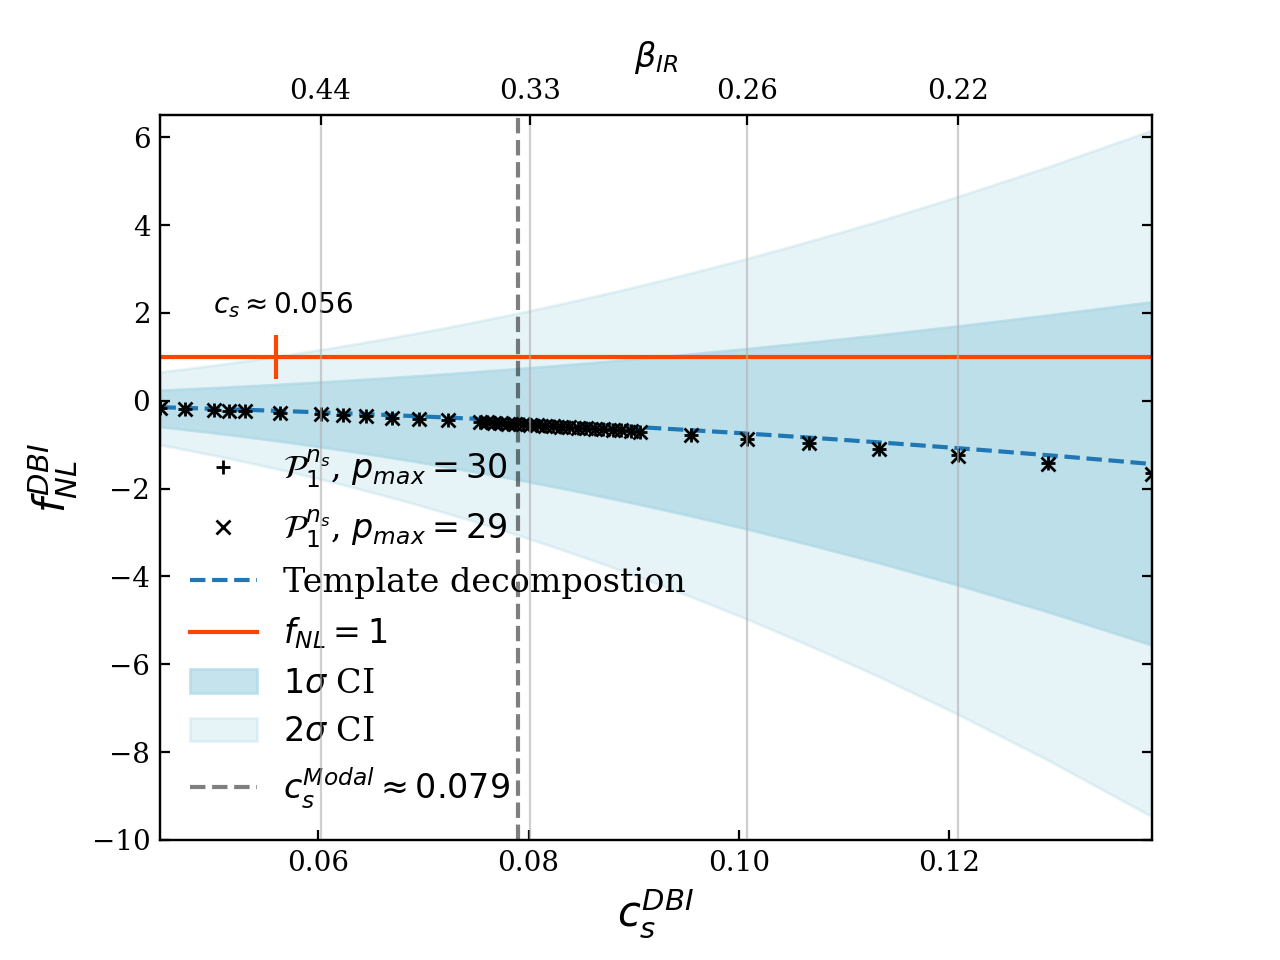
\includegraphics[width=0.9\textwidth]{wuhyun_plots/beta_ir_constraint_busy.png}
        \caption{
            \textcolor{red}{To replace the above---need to make less cramped!
            Note that the $\beta_{IR}$ scale is not linear!}
            Our constraint on DBI inflation. Here $c_s^{DBI}$ is not an input parameter
            (unlike in the template case), instead it is time dependent, and the plotted
            value is taken from the horizon crossing of the pivot scale. We find that $\beta_{IR}<0.5$
            %0.464
            is outside of our $2\sigma$ confidence interval. This plot was obtained by
            scanning across values of $\beta_{IR}$ and calculating the corresponding primordial bispectra
            using $\primodal$, then projecting those bispectra onto the $\cmb$
            and comparing them to the $\planck$ $\cmb$ temperature data using
            $\cmbbest$. Since the amplitude is fixed by the scenario, we rule out a
            scenario by ruling out $f_{NL}^{DBI}=1$.
            Note that the constraint obtained for $\Pmax=30$ and $\Pmax=29$ is identical,
            so we can be confident that our constraint has converged in $\Pmax$.
            We can see that the $\cmbbest$ result does not agree with the $\modal$ result,
            but as we see in figure~\ref{fig:equil_constraints_comparison},
            the discrepancy is not unexpected. We discuss possible explanations
            \textcolor{red}{in the text}.
        }\label{fig:dbi_sound_speed_scan_beta}
    \end{figure}
    \begin{figure}[htbp!]
        \centering
        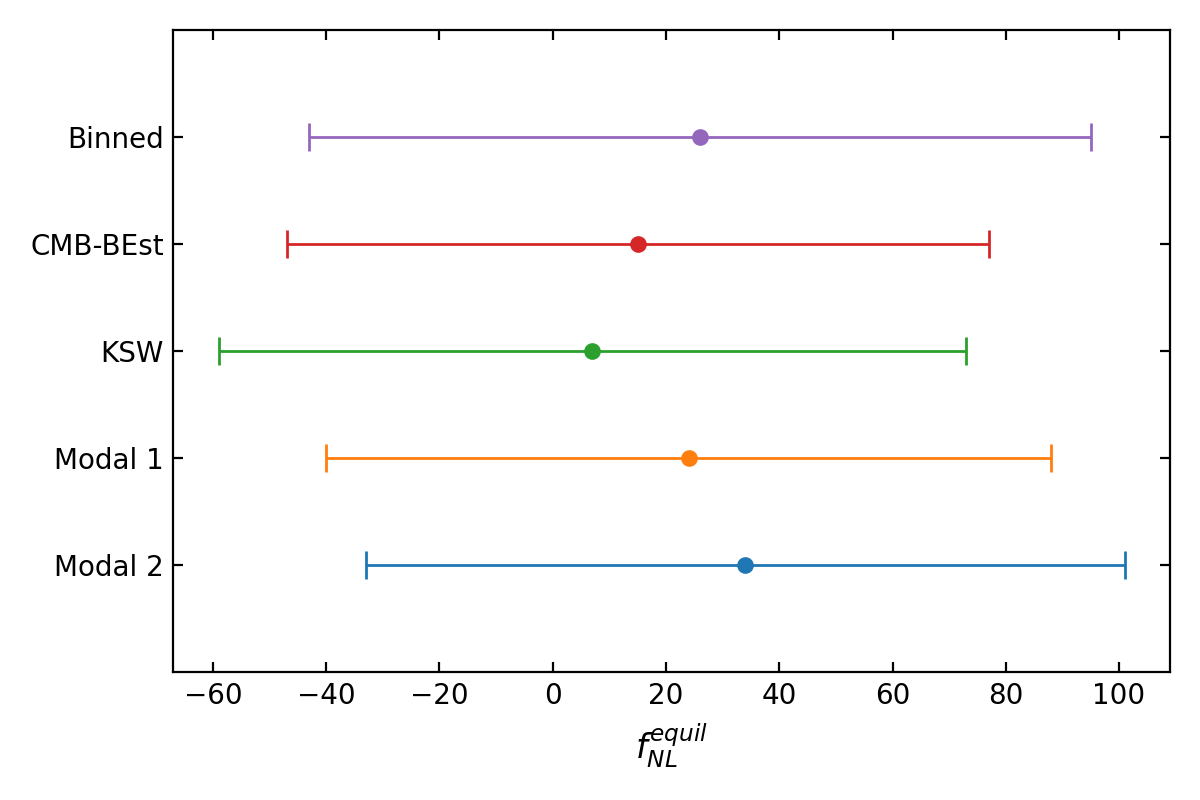
\includegraphics[width=0.9\textwidth]{wuhyun_plots/fnl_equil_planck_scatter.png}
        \caption{
            A comparison of the various estimation methods used in $\planck$
            (as presented in table 5 of~\cite{Planck_NG_2018}).
            We plot the constraints obtained by each method for $\fnlequil$,
            as well as the constraint obtained by $\cmbbest$ (presented in~\cite{Sohn_2021})
            along with their $68\%$ uncertainty margin.
            We see that while the estimators do not agree, there is no discrepancy with any
            significance---in particular, we see that $\cmbbest$ is not an outlier.
            The $\cmbbest$ result quoted here was obtained by decomposing the equilateral
            template~\eqref{equil_shape} (using definition~\eqref{planck_fnl_defn_ns} for $\fnlequil$)
            in the $\Lnsinv$ basis for $\Pmax=30$.
        }\label{fig:equil_constraints_comparison}
    \end{figure}

\section{Slow-roll effects}
    Here we will compare template decompositions to Primodal results.
    This will tell us how large the slow-roll corrections are to the
    final CMB result, but not anything about the primordial convergence.
    The main slow-roll corrections are a correction to the amplitude,
    and a deviation from perfect scale-dependence.
%\section{EFT stuff, build off Enrico's recent work.}
%    Words
